\documentclass[10pt,a4paper]{article}
\usepackage[T1]{fontenc}
\usepackage{lmodern}
\usepackage[margin=1.8cm]{geometry}
\usepackage{booktabs}
\usepackage{tabularx}
\usepackage{array}
\usepackage{graphicx}
\usepackage{xcolor}
\usepackage{amsmath}
\usepackage{enumitem}
\usepackage{fancyhdr}
\usepackage[hidelinks]{hyperref}
\usepackage{caption}
\usepackage{float}

\definecolor{Navy}{HTML}{17324D}
\definecolor{Green}{HTML}{147A5B}
\definecolor{Gold}{HTML}{D49B2A}
\definecolor{Light}{HTML}{F1F4F6}
\definecolor{Gray}{HTML}{667788}
\definecolor{Red}{HTML}{B54242}

\hypersetup{colorlinks=true,linkcolor=Navy,urlcolor=Green}
\setlength{\parindent}{0pt}
\setlength{\parskip}{5pt}
\setlist[itemize]{leftmargin=1.3em,itemsep=2pt,topsep=2pt}
\renewcommand{\arraystretch}{1.15}
\newcolumntype{L}[1]{>{\raggedright\arraybackslash}p{#1}}
\newcolumntype{Y}{>{\raggedright\arraybackslash}X}

\pagestyle{fancy}
\fancyhf{}
\lhead{\color{Gray}\small TSP free-acid modeling}
\rhead{\color{Gray}\small Model upgrade addendum}
\cfoot{\color{Gray}\small \thepage}
\renewcommand{\headrulewidth}{0.3pt}

\newcommand{\good}[1]{\textcolor{Green}{\textbf{#1}}}
\newcommand{\warn}[1]{\textcolor{Gold}{\textbf{#1}}}
\newcommand{\statusbox}[1]{\colorbox{Light}{\parbox{0.96\linewidth}{#1}}
}

\begin{document}

\begin{titlepage}
  \color{Navy}
  \vspace*{2.3cm}
  {\Huge\bfseries SLURRY\_FREE\_ACID Modeling\par}
  \vspace{0.35cm}
  {\LARGE Model Upgrade Addendum\par}
  \vspace{0.7cm}
  {\large Work completed after the first project advancement report\par}
  \vspace{1.0cm}
  {\large Prepared by: Ikram Benfellah\par}
  \vfill
  \statusbox{\textbf{Main result:} the target-free Ridge--LightGBM model was improved retrospectively and a regime-aware hybrid reduced forward-validation fragility. The two candidates have different strengths; neither is externally validated because only the January month is available.}
  \vfill
  {\large Internship project\hfill 17 August 2026}
  \vspace{0.3cm}
  \color{Gold}\rule{\textwidth}{4pt}
\end{titlepage}

\section*{Executive summary}

After the first report, I focused on improving the \textbf{target-free virtual sensor}: process measurements are used to estimate the current free-acid value without using current or historical \texttt{SLURRY\_FREE\_ACID} as an input.

I completed two additional notebooks:
\begin{itemize}
  \item \textbf{Notebook 06:} compared recency weighting, clustered local experts, stronger Ridge regularization, LightGBM alternatives, and Ridge--LightGBM blends using four expanding validation blocks;
  \item \textbf{Notebook 07:} combined the global blend with five local Ridge experts to test whether operating-region specialization improves robustness.
\end{itemize}

\begin{tabularx}{\textwidth}{L{0.25\textwidth}L{0.18\textwidth}L{0.18\textwidth}Y}
\toprule
\textbf{Candidate} & \textbf{Mean validation RMSE} & \textbf{Worst-block RMSE} & \textbf{Decision} \\
\midrule
Notebook 06 global 50/50 blend & 0.3201 & 0.4124 & Accuracy-oriented candidate; retrospective test RMSE 0.2879. \\
Notebook 07 80\% local hybrid & 0.3217 & \textbf{0.3520} & Robustness-oriented candidate; retrospective test RMSE 0.2889. \\
\bottomrule
\end{tabularx}

\statusbox{\textbf{Decision:} keep both candidates frozen. Notebook 06 is slightly better on the already-inspected test period. Notebook 07 is more stable across forward validation blocks. A genuinely later labeled month is required to choose between them.}

\section{Scope retained from the first report}

The original experimental design was not changed:
\begin{itemize}
  \item the preparation layer and Feature Set D are inherited from Notebook 02;
  \item timestamps remain chronological and data are never shuffled;
  \item preprocessing is fitted inside each training fold only;
  \item the target, future-target columns, and target history are absent from the model inputs;
  \item January's final test period is reported as \textbf{retrospective}, because it was already inspected previously.
\end{itemize}

The three operational cases from the first report remain separate:
\begin{itemize}
  \item direct future-level forecasting;
  \item target-anchored change forecasting when $y_t$ is available;
  \item target-free current-value estimation when no free-acid measurements are supplied.
\end{itemize}

The new work concerns only the third case.

\section{Notebook 06: controlled target-free upgrades}

\subsection*{Question}

Could a compact adaptation method improve the process-only virtual sensor without introducing target leakage or unnecessary sequence-model complexity?

\subsection*{Models tested}

\begin{tabularx}{\textwidth}{L{0.24\textwidth}Y L{0.29\textwidth}}
\toprule
\textbf{Method} & \textbf{Purpose} & \textbf{Executed choices} \\
\midrule
Global Ridge & Stable regularized linear reference & $\alpha=10$ and 100; median imputation and standard scaling \\
Recency-weighted Ridge & Give recent process states more influence & Half-lives of 3, 7, and 14 days \\
Clustered Ridge experts & Fit separate linear relationships in data-defined operating regions & KMeans with 3 or 5 clusters; one Ridge expert per cluster \\
LightGBM & Learn nonlinear thresholds and interactions & 150 trees; 15 or 31 leaves; learning rate 0.05 \\
Ridge--LightGBM blend & Combine linear stability and nonlinear flexibility & Ridge weights 0.3, 0.5, and 0.7 \\
\bottomrule
\end{tabularx}

\subsection*{Validation design}

The original validation interval was divided into four consecutive blocks. For each block, the training set contained the original training data plus only the earlier validation blocks.

\begin{tabularx}{\textwidth}{L{0.08\textwidth}L{0.15\textwidth}L{0.17\textwidth}Y}
\toprule
\textbf{Block} & \textbf{Training rows} & \textbf{Validation rows} & \textbf{Validation period} \\
\midrule
1 & 30,940 & 1,657 & 22 Jan 17:18 to 23 Jan 21:08 \\
2 & 32,597 & 1,657 & 23 Jan 21:09 to 25 Jan 00:49 \\
3 & 34,254 & 1,657 & 25 Jan 00:50 to 26 Jan 04:30 \\
4 & 35,911 & 1,657 & 26 Jan 04:31 to 27 Jan 08:58 \\
\bottomrule
\end{tabularx}

Selection was based on candidates within 2\% of the best mean RMSE, followed by the lowest worst-block RMSE and RMSE standard deviation. The test period was not used for this decision.

\subsection*{Executed results}

\begin{tabularx}{\textwidth}{Y L{0.16\textwidth}L{0.16\textwidth}L{0.15\textwidth}}
\toprule
\textbf{Candidate} & \textbf{Mean RMSE} & \textbf{RMSE SD} & \textbf{Worst RMSE} \\
\midrule
70\% Ridge / 30\% LightGBM & \textbf{0.3191} & 0.0762 & 0.4236 \\
50\% Ridge / 50\% LightGBM & 0.3201 & 0.0686 & 0.4124 \\
Five-cluster Ridge & 0.3280 & \textbf{0.0396} & \textbf{0.3522} \\
Global Ridge, $\alpha=100$ & 0.3274 & 0.0811 & 0.4353 \\
LightGBM, 31 leaves & 0.3483 & 0.0599 & 0.4080 \\
\bottomrule
\end{tabularx}

The selected candidate was the 50/50 Ridge--LightGBM blend. Compared with the Notebook 05 frozen blend, refitting on training plus validation reduced retrospective test RMSE from 0.3014 to 0.2879 and MAE from 0.2490 to 0.2344. This is a 4.48\% RMSE reduction, but it is not fresh external evidence.

\textbf{Interpretation}
\begin{itemize}
  \item Recency weighting did not improve performance; simple exponential down-weighting was not sufficient.
  \item LightGBM alone was weaker than the blend.
  \item The five-cluster Ridge model was more stable, which motivated Notebook 07.
  \item The retrospective gain mainly reflects stronger validation and refitting with more development data, not a completely new architecture.
\end{itemize}

\begin{figure}[H]
\centering
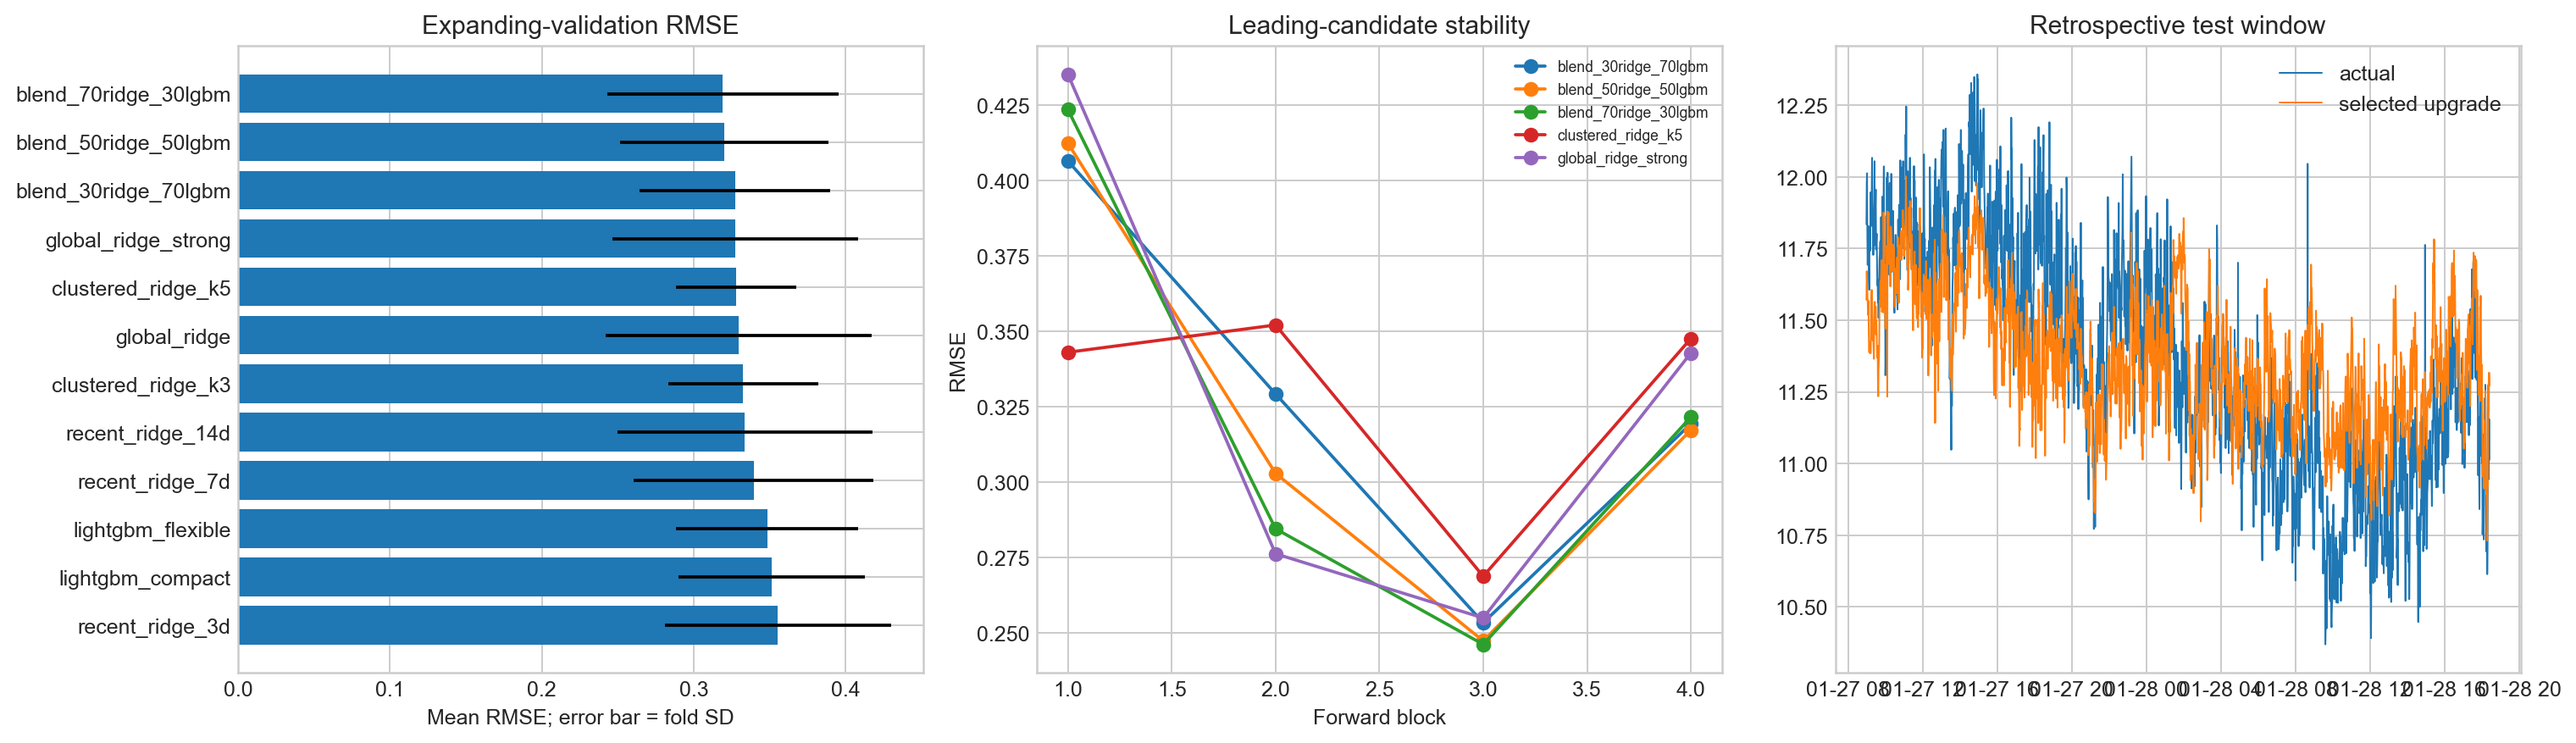
\includegraphics[width=\textwidth]{target_free_upgrade_artifacts/figures/upgrade_benchmark.png}
\caption{Notebook 06 benchmark. The left panel compares mean expanding-validation RMSE, the center shows time-block variability, and the right panel is the already-inspected retrospective test window.}
\end{figure}

\section{Notebook 07: regime-aware hybrid}

\subsection*{Question and implementation}

Notebook 06 showed a trade-off: the global blend had better average accuracy, while local Ridge experts had a better worst block. I therefore combined both components.

For each validation fold:
\begin{itemize}
  \item median imputation and standard scaling were fitted on the fold's training rows;
  \item the global prediction was
  \[
    \hat y_{\mathrm{global}}=0.5\hat y_{\mathrm{Ridge}}+0.5\hat y_{\mathrm{LightGBM}};
  \]
  \item KMeans divided the standardized training rows into five data-defined regions;
  \item one Ridge expert was fitted per region, with a global Ridge fallback for regions containing fewer than 100 training rows;
  \item fixed local weights from 0.0 to 1.0, in steps of 0.1, were evaluated;
  \item distance gates at the 50th, 70th, 85th, and 95th percentiles were also evaluated.
\end{itemize}

The fixed hybrid is
\[
\hat y=(1-w)\hat y_{\mathrm{global}}+w\hat y_{\mathrm{local}}.
\]
KMeans clusters are statistical operating regions, not confirmed production regimes.

\subsection*{Main validation results}

\begin{tabularx}{\textwidth}{Y L{0.15\textwidth}L{0.15\textwidth}L{0.15\textwidth}}
\toprule
\textbf{Local weight} & \textbf{Mean RMSE} & \textbf{RMSE SD} & \textbf{Worst RMSE} \\
\midrule
0.0 - global only & 0.3201 & 0.0686 & 0.4124 \\
0.4 - best mean & \textbf{0.3160} & 0.0522 & 0.3777 \\
0.5 & 0.3165 & 0.0487 & 0.3703 \\
0.8 - selected & 0.3217 & 0.0412 & 0.3520 \\
1.0 - local only & 0.3280 & \textbf{0.0396} & 0.3522 \\
\bottomrule
\end{tabularx}

The 40\% local blend had the best mean RMSE. The stability-first rule selected the 80\% local blend because its mean remained within 2\% of the best and it had the lowest worst-block RMSE in that pool.

Relative to the global-only model, the selected hybrid:
\begin{itemize}
  \item changed mean RMSE from 0.3201 to 0.3217: approximately 0.5\% worse;
  \item reduced worst-block RMSE from 0.4124 to 0.3520: approximately 14.7\% better;
  \item reduced RMSE standard deviation from 0.0686 to 0.0412: approximately 39.9\% lower;
  \item reduced mean MAE from 0.2546 to 0.2500.
\end{itemize}

\subsection*{Retrospective comparison}

\begin{tabularx}{\textwidth}{Y L{0.16\textwidth}L{0.16\textwidth}L{0.14\textwidth}}
\toprule
\textbf{Candidate} & \textbf{Test MAE} & \textbf{Test RMSE} & \textbf{Test $R^2$} \\
\midrule
Notebook 06 global blend & 0.2344 & \textbf{0.2879} & \textbf{0.5970} \\
Notebook 07 selected hybrid & \textbf{0.2309} & 0.2889 & 0.5941 \\
\bottomrule
\end{tabularx}

The hybrid improved MAE slightly but increased RMSE by 0.36\%. This indicates a different error distribution, not a clear overall win.

\begin{figure}[H]
\centering
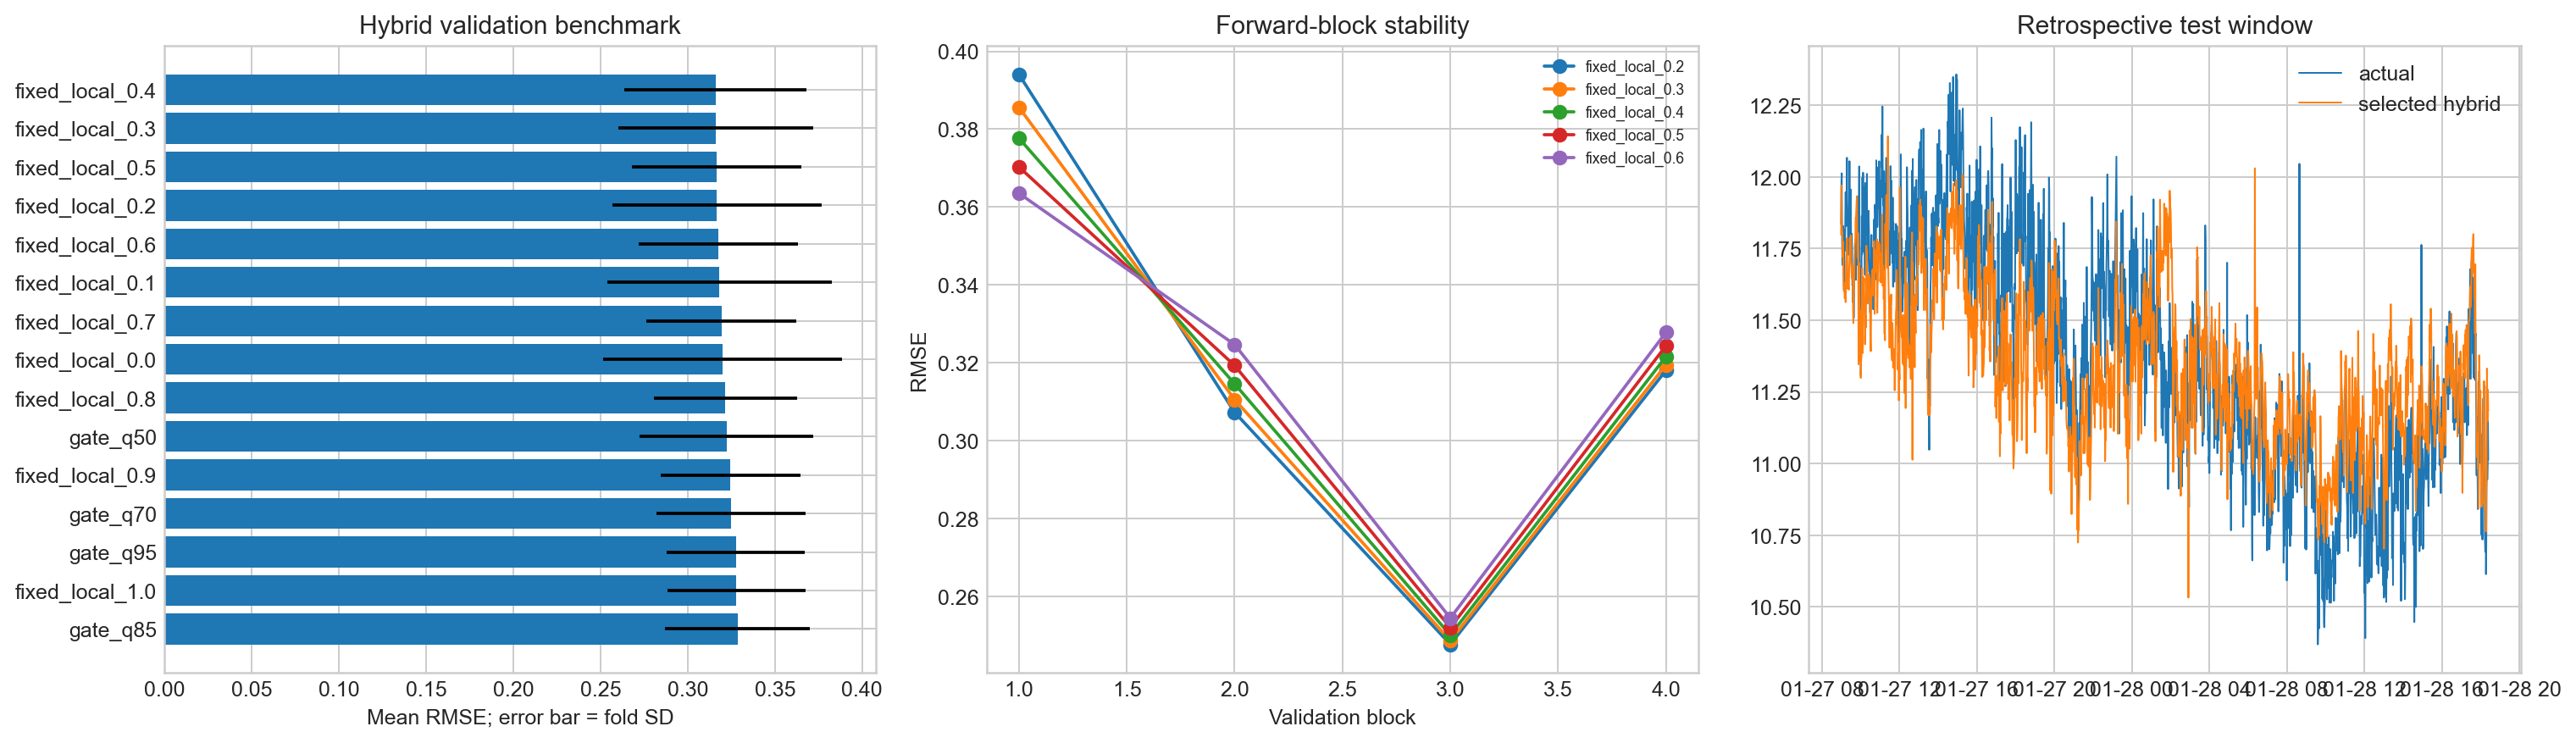
\includegraphics[width=\textwidth]{regime_aware_hybrid_artifacts/figures/regime_aware_hybrid_benchmark.png}
\caption{Notebook 07 results. Fixed blends gave a better mean/stability trade-off than hard distance gates. The test trace is retrospective and is not used for selection.}
\end{figure}

\section{Engineering interpretation and limitations}

\begin{itemize}
  \item \textbf{Average accuracy and robustness are different objectives.} The best mean model is not the model with the best worst-period performance.
  \item \textbf{Local structure is present, but not yet physically labeled.} Some KMeans regions had no rows in particular validation blocks, showing that operating coverage changes with time.
  \item \textbf{Hard distance gating was not superior.} Smooth fixed blending was more reliable than switching abruptly between global and local predictions.
  \item \textbf{Only one month is available.} Adjacent one-minute samples are not equivalent to independent months or production campaigns.
  \item \textbf{The January test is no longer untouched.} It cannot support a final model replacement claim.
  \item \textbf{No causal or control recommendation follows from these models.} The variable registry and process-engineer confirmation remain mandatory.
\end{itemize}

\section{Final model status}

\begin{tabularx}{\textwidth}{L{0.25\textwidth}Y Y}
\toprule
\textbf{Role} & \textbf{Current candidate} & \textbf{Reason} \\
\midrule
Accuracy-oriented target-free model & Notebook 06 50/50 Ridge--LightGBM & Lowest retrospective RMSE and stronger $R^2$ \\
Robustness-oriented target-free model & Notebook 07 80\% local hybrid & Much lower worst-block RMSE and variability \\
Mean-validation alternative & Notebook 07 40\% local hybrid & Lowest mean expanding-validation RMSE \\
Operational model & Not selected & Requires a genuinely later labeled month \\
\bottomrule
\end{tabularx}

All Notebook 07 readiness checks passed:
\begin{itemize}
  \item no target or target-history input;
  \item four chronological forward blocks and no shuffle;
  \item preprocessing fitted inside each fold;
  \item test excluded from candidate selection;
  \item model bundle, predictions, tables, diagnostics, and readiness files exported.
\end{itemize}

\section{Next work}

\begin{enumerate}[leftmargin=1.5em,itemsep=3pt]
  \item Obtain at least one later month containing process variables and measured \texttt{SLURRY\_FREE\_ACID}.
  \item Freeze Notebook 06 and Notebook 07 candidates before loading that month.
  \item Compare RMSE, MAE, bias, drift, transition errors, and missing-sensor behavior without retuning.
  \item Ask the process team whether the KMeans regions correspond to known grades, production rates, startups, shutdowns, or equipment states.
  \item Select one operational candidate only if its improvement is consistent across months and practically meaningful.
  \item Recalibrate prediction intervals and dashboard drift thresholds on multi-month data.
\end{enumerate}

Deep sequence models should remain deferred until several chronological months are available. With the current data, external generalization and regime coverage are more important than adding model complexity.

\section*{Addendum change log}

This addendum adds the work not present in the first advancement report:
\begin{itemize}
  \item expanding four-block model validation;
  \item recency-weighted and clustered target-free alternatives;
  \item the revised Ridge--LightGBM retrospective result;
  \item fixed and distance-gated global/local hybrids;
  \item the explicit accuracy-versus-robustness decision;
  \item the requirement for a new external month before model replacement.
\end{itemize}

\end{document}
